\subsection{Validação do modelo}
A tarefa alvo do modelo final é classificar em qual das Sete Expressões Faciais Universais pertence determinada expressão facial dada como entrada a imagem de uma face. Observando o problema a ser resolvido, percebe-se que este é de natureza classificatória. Na literatura, os problemas dessa natureza tem seu desempenho comumente avaliados via Matriz de Confusão e também da via medida \emph{F}. Onde a medida \emph{F} escolhida foi a \emph{F1 Micro}, devido a natureza desbalanceada da base de dados \cite{}.

Para validação do \emph{XGBoost} foi utilizado a validação cruzada estratificada \cite{}, para que o desbalanceamento das classes na base de dados fosse replicada nas partições. O número de partições recomendado pela literatura é dez \cite{}, contudo, este valor é sugerido para base de dados grandes, o que não reflete a realidade da escolhida. Para a validação deste modelo foi escolhido sete partições, pois, o conjunto \emph{PrivateTest} é aproximadamente $\frac{1}{8}$ da base de dados, o que deixa $\frac{7}{8}$ a serem divididos na validação cruzada. Ressaltando que o conjunto \emph{PrivateTest} foi mantido fixo e utilizado somente como validação final do modelo, para que a comparação com os resultados da competição no \emph{Kaggle} fosse realizada.

Na Figura \ref{fig:datasetSplit} é possível visualizar a separação original da base de dados, divida em 8 partes de mesmo tamanho, e também é possível observar a separação utilizada na validação cruzada, respectivamente na primeira e segunda linha.

\begin{figure}[!htb]
    \centering
    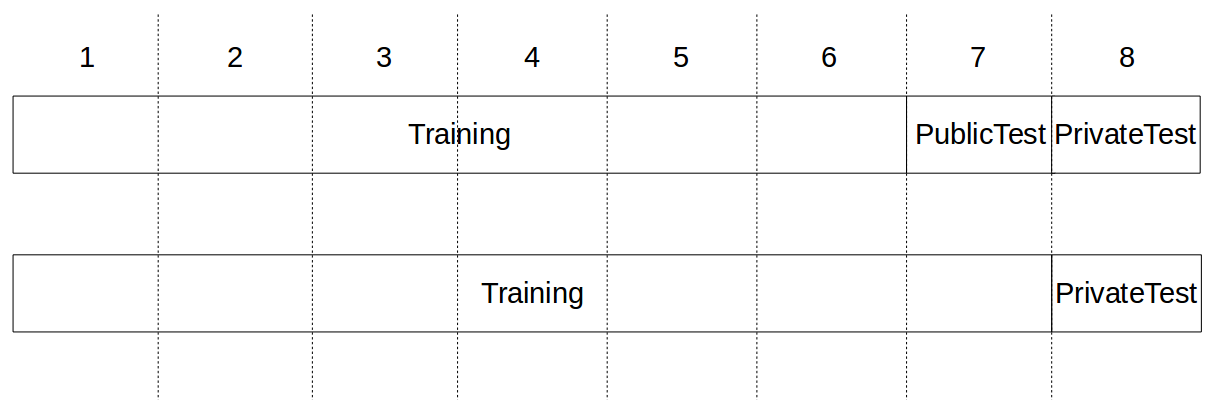
\includegraphics[width=15cm]{images/evaluation.png}
    \caption{Separação de exemplos da base de dados para Treinamento, Validação e Teste.}
    \label{fig:datasetSplit}
\end{figure}